\chapter{绪论}
\label{ch:introduction}

% 宇宙中可见的物质含量不足以解释所观测到的星系内部以及星系之间彼此产生的引力强度。这就导致了科学家猜测宇宙中有含量多达90%的物质都属于不会辐射电磁波也不会与普通重子物质相互作用的暗物质。
在宇宙学中,暗物质(Dark Matter)是指无法通过电磁波的观测进行研究,也就是不参与电磁相互作用的一类物质形式。
虽然暗物质的属性还不是很明确,但暗物质具有引力相互作用,能够干扰星体发出的光波,从而影响宇宙大尺度结构,因此大量的天文观测结果已经证明了暗物质的存在。
如今,暗物质假说被大多数天文学家所接受,并在大爆炸宇宙学模型,星系的形成与演化模型以及对宇宙微波背景辐射各向异性的解释中扮演重要角色。

最新的研究结果表明\parencite{planck_collaboration_planck_2014},宇宙的能量物质组成中\SI{68.3}{\percent}是暗能量,\SI{26.8}{\percent}是暗物质,而普通物质只占\SI{4.9}{\percent}。这意味着,暗物质在宇宙全部物质质量中占据了\SI{84.5}{\percent},远远超过了能够被“看到”的普通物质含量。
然而,人们对这部分占主导地位的宇宙成分的理解还仅仅来自于宇宙大尺度结构的观测结果,而对暗物质的组成成分以及性质这类更加细致的问题还知之甚少。
现有的理论模型也不能对暗物质的属性问题给出很好的解释,特别的,在粒子物理学中成功解释了大部分实验结果并给出过精确预言的标准模型(Standard Model)并不包含一个可行的暗物质候选粒子方案,即在标准模型中找不到符合所有已知的暗物质性质的粒子类型。
暗物质这种不能够被现有理论解释的新现象大大激发了科学家们的研究兴趣,它和暗能量一起被称为是笼罩着21世纪物理学的两朵“乌云”。
暗物质粒子探测是当前的科学热点, 具有重要的物理意义和前景, 世界各国都在集中人力、物力和财力研究这一问题。
就像一个多世纪前的两朵“乌云”催生了现代物理学的基础:量子力学和相对论一样,对暗物质粒子的探测和研究很可能导致物理学产生新的革命。

随着科学技术的进步,近年来对暗物质的探测研究渐渐向精确测量方向发展。
暗物质粒子探测卫星(DArk Matter Particle Explorer,简称DAMPE)是中国科学家独立提出并自主研制的空间暗物质探测项目,它于2015年12月17日成功发射并进入预定轨道。
DAMPE是目前世界上观测能段范围最宽、能量分辨率最优的空间暗物质粒子探测器,它的成功发射不仅标志着我国在空间暗物质探测领域占有了一席之地,而且将为今后的暗物质研究提供更多新的有价值的观测数据,为解决暗物质之迷提供助力。

\section{暗物质研究的现状}
\subsection{暗物质存在的证据:宇宙大尺度结构的观测结果}
暗物质的存在已经被各个宇宙学尺度的天文观测结果所证实。
下面依次从星系尺度范围(Galactic Scale),星系团尺度范围(The Scale of Galaxy Clusters)和宇宙尺度范围(Cosmological Scale)三个方面,对一些能够证明暗物质存在的典型证据进行介绍。

在星系尺度范围,暗物质存在最令人信服和直接的证据来自于星系旋转曲线或(Galaxy Rotation Curve,也叫作星系自转曲线)的观测结果。
星系旋转曲线是指星系中的恒星或气体的轨道速度$V(r)$与它们距离星系中心的距离$r$之间的关系曲线。
根据开普勒定律,在距离星系质量中心区域很远的恒星或气体,其轨道速度应该满足$V(r)\propto 1/\sqrt{r}$,即距离星系中心的越远,它们的轨道速度就越小;
而对大量旋转星系的观测\parencite{rubin1980rotational}却发现,其内部星体的轨道速度并没有出现预期的随距离平方根减小,而是表现得较为平坦,如图\ref{fig:introduction:rotation_curve}所示。
\begin{figure}[htbp]
	\centering
	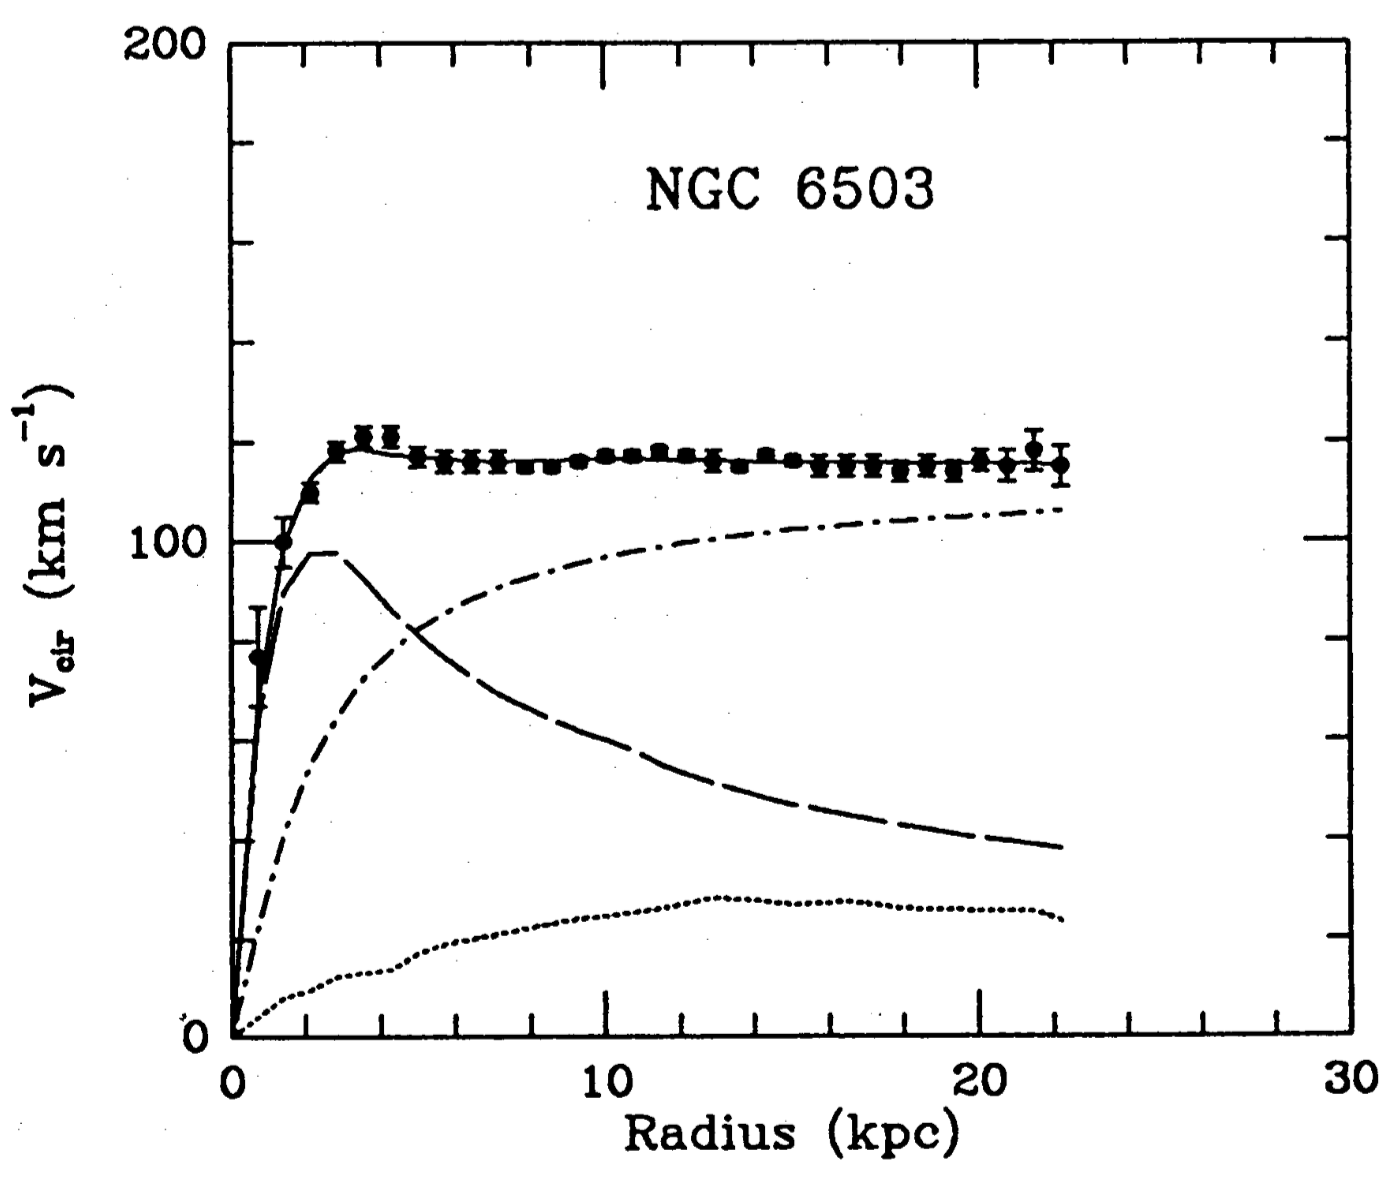
\includegraphics[width=0.65\textwidth]{chap/introduction/fig/rotation_curve.png}
	\caption{一个典型的星系旋转曲线,引自\parencite{begeman_extended_1991}。其中黑色方块是观测值,虚线代表可见物质的贡献,点线代表气体的贡献,点虚线是暗物质晕(dark matter halo)的贡献,而实现是三种成分的组合。}
	\label{fig:introduction:rotation_curve}
\end{figure}
这个现象表明,星系内部存在大量的“不可见”物质:暗物质晕,它们弥漫在星系可见质量中心的周围,并通过引力作用拉住星系外侧的组成,以使其不致因过大的离心力而脱离星系\parencite{bosma1978distribution}。
星系旋转曲线的异常现象使得“暗物质”这个概念被科学界普遍接受。

实际上,现代意义上的“暗物质”概念由瑞士天文学家F.Zwicky在1933年研究星系团内的星系运动时首次提出来的\parencite{zwicky1933spectral}。
Zwichy根据测得的Coma星系团内星系运动的速度弥散(Velocity Dispersion),应用维里定理得到了该星系团的质光比(Mass-to-light Ratio),发现它比太阳附近的质光比要大两个量级,即Coma星系团内可见部分的质量只占根据万有引力效应测得的星系团总质量的一小部分。
据此,Zwichy认为存在着未被人们观测到的质量缺失,他将这些缺失的质量称之为“暗物质”,然而这在当时并没有引起人们的重视。
如今,有许多办法可以测定星系团的质量,如通过弱引力透镜效应,通过测团内热气体的X射线发射轮廓图以及通过测量径向速度分布等。
特别的,美国天文学家在2006年利用钱德拉X射线望远无意间观测到了Bullet星系团的碰撞过程\parencite{bullet_cluster},得到了迄今为止能够证明暗物质存在的最直接证据和最有说服力的证据。
在大部分时候,由于引力作用导致的相互吸引,宇宙中的暗物质和可见物质是掺杂在一起的。
而Bullet星系团由一大一小两个正在碰撞中的星系团组成,两个星系团之间的碰撞如此剧烈,以致暗物质和正常物质分离开来并被观测到,如图\ref{fig:introduction:bullet_cluster}所示。
\begin{figure}[htbp]
	\centering
	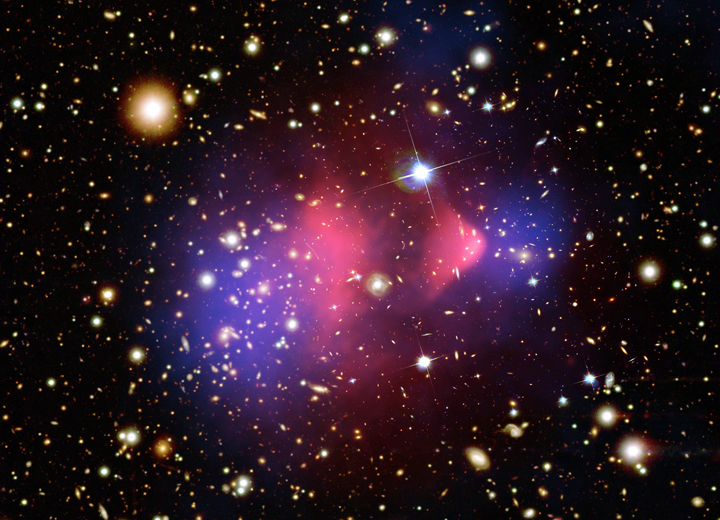
\includegraphics[width=0.65\textwidth]{chap/introduction/fig/bullet_cluster.jpg}
	\caption{Bullet星系团的碰撞过程\parencite{bullet_cluster}}
	\label{fig:introduction:bullet_cluster}
\end{figure}
图中红色部分是钱德拉X射线望远镜得到的Bullet星系团中的可见物质质量分布,而蓝色部分是根据哈勃望远镜的观测结果,利用引力透镜效应反推得到的Bullet星系团中的全部物质质量分布。
一方面,可见物质由于相互间的电磁相互作用,它们在碰撞后的分离速度小于不受电磁相互作用制约的暗物质分离速度;另一方面,暗物质所占的质量比例又远大于可见物质的质量比例。
上述两个因素合在一起,最终导致了Bullet星系团中全部质量的中心与可见物质质量中心的分离。

星系和星系团尺度的观测结果能够证明暗物质的存在,但却不够给出宇宙中暗物质所占的比例,这部分信息是从宇宙微波背景辐照(Cosmic Microwave Backgroud)的观测结果中提取出来的。
在大爆炸发生约38万年后,由于宇宙的膨胀冷却,使得电子和质子能够结合形成氢原子,并在这个过程中会放射出大量的光子。
这些光子大部分能够不受干扰地传播到现在并被我们观测到,虽然它们在产生时的频率为紫外波段,但宇宙加速膨胀引起的红移使得它们的频率在今天被观测到时处于微波波段,这就是宇宙微波背景辐射。
宇宙微波背景辐射各向异性反映了宇宙历史早期的温度涨落,对它的精确观测能够验证宇宙学模型并严格限制各种宇宙学参数\parencite{bertone_particle_2005},其中包括暗物质的质量比例。
图\ref{fig:introduction:planck_power_law}给出了Planck卫星测得的角功率谱,其中三个主峰的面积依次代表了暗能量、普通物质以及暗物质的相对比例,这也是我们常说的宇宙能量物质组成比例的由来。
\begin{figure}[htbp]
	\centering
	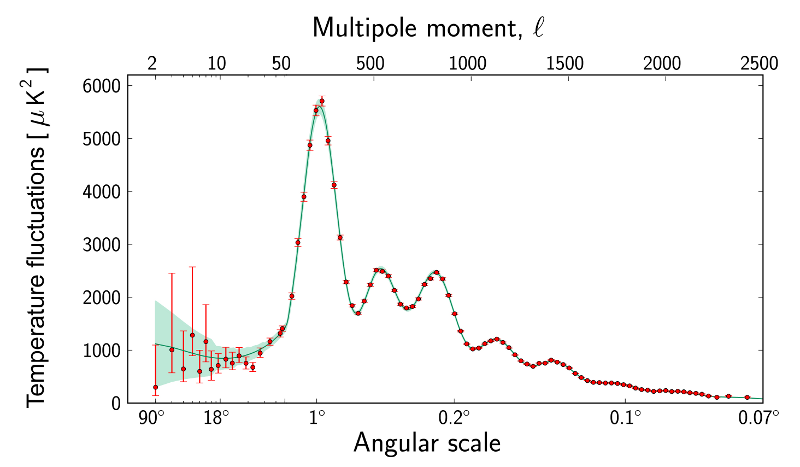
\includegraphics[width=0.8\textwidth]{chap/introduction/fig/planck_power_law.png}
	\caption{Planck卫星测到的角功率谱,引自\parencite{planck_collaboration_planck_2014}}
	\label{fig:introduction:planck_power_law}
\end{figure}

\subsection{暗物质的粒子属性:标准模型之外的物理}
虽然暗物质的存在已经得到了上述天文实验观测的证实, 但暗物质性质和组成成分仍然不为人们所了解。
早期暗物质的理论着重在一些很难被观测到的一般物质星体,例如:黑洞、中子星、衰老的白矮星、褐矮星等,这些星体一般被统称为晕族大质量致密天体(MAssive Compact Halo Objects,简称为MACHOs)。
然而,多年來的天文观测并没有找到足量的MACHOs以符合观测到暗物质质量比例\parencite{tisserand_limits_2007}。
一般认为,难以探测的重子物质(如MACHOs)确实贡献了部分的暗物质组成,但这类物质只占了其中的一小部分\parencite{freese_death_2000}。
暗物质主要组成成分应该是所谓的非重子暗物质(Non-baryonic Dark Matter),这类非重子暗物质是由一种或多种不同于一般物质(电子、质子、中子、中微子等)的基本粒子所构成,因此也常被叫做暗物质粒子。

非重子暗物质的候选粒子种类非常多,如轴子(Axion),KK粒子,超对称引力子(gravitino),超对称精质场(quintessino)等等\parencite{bixiaojun}。
其中,最热门也是最有希望的是所谓的弱相互作用重粒子 (Weakly Interacting Massive Particles,简称WIMP),如超对称粒子或额外维空间粒子等。
WIMP粒子满足暗物质粒子必须的基本性质:1)暗物质粒子是稳定的或者寿命较长,其寿命至少相当于宇宙年龄尺度;2)暗物质粒子的质量比一般基本粒的子要大,且具有引力相互作用;3)通常认为暗物质粒子不发生电磁相互作用,即便有其强度也应该低于或相当于弱相互作用强度;4)从宇宙结构形成理论出发推知,当暗物质脱耦时,它应该是“冷”的(非相对论性的),即脱耦温度远小于 暗物质粒子质量。

然而,标准模型中并不存在符合上述所有性质的稳定WIMP粒子。
另一反面,许多设法理解电弱对称破缺机制的所谓超出标准模型的新物理理论都提供了这样的WIMP粒子,比 如超对称理论(SUpper-SYmmetry,简称SUSY)中最轻的超对称粒子(Neutralino)以及额外维空间理论所预言的KK粒子。
如果我们发现了某种新物理所预言的粒子并符合暗物质粒子的基本性质,它很可能就是构成暗物质的粒子;反过来,如果暗物质粒子被探测到,其性质也会限制新物理的形式。
总之,对暗物质粒子的研究将会大大拓展人们对未知世界的了解,并可能产生新的突破。

\subsection{暗物质粒子的探测:精细测量时代的到来}
暗物质的存在证据最开始只是天文观测结果的附属产品。
近年来,随着对暗物质的理解越来越深刻,人们不再满足于原有的具有极大限制性的天文观测方法,开始采用新的探测手段对暗物质进行更加细致的研究。
如今,探测暗物质粒子的方法大致可以总结为三类:加速器直接产生法,直接探测法和间接探测法。
下面,依次对这三种方法进行简单的介绍。

加速器直接产生法是发现新粒子最常用和最有效的方法。
利用加速器将粒子加速到高能量进行对撞可以模拟宇宙大爆炸初期环境,各种新的粒子能够在对撞后产生,其中也可能包含暗物质粒子。
通过对次级粒子的探测或逃逸能量(missing energy)的重建,可以反推出新粒子的存在并在实验室环境下研究粒子的物理特性。
产生暗物质粒子需要极高的能量,目前只有欧洲核子中心的大型强子对撞机(Large Hadron Collider,简称LHC)以及计划中的国际直线对撞机(International Linear Collider,简称ILC)能够满足这个条件。
然而,加速器方法只能产生较轻的暗物质粒子,对于更重的暗物质候选粒子,需要建造更高能量的加速器和更加强大的粒子探测器,因此具有较大的局限性。

直接探测方法是目前最重要也是最常被采用的暗物质粒子探测方式,其基本原理与中微子的探测基本一致:银河系中充满了暗物质粒子并且不断地穿过地球,通过捕捉暗物质粒子与探测器介质原子核相互作用产生的光学、声学以及电子学信号来可以对暗物质粒子进行研究。
由于暗物质粒子与普通物质的反应截面非常小,这类探测设备一般需要使用成吨的探测介质,并需要对背景事例进行细致的研究。
为了屏蔽来自宇宙线的背景事例,实验装置一般都安置在极深的地下,同时对使用的材料纯度具有极高的要求。
目前, 世界上有二十几家使用直接探测方法的实验正在运行或即将投入运行,相关的探测技术也在不断发展更新中,然而直到现在仍然没有确切的暗物质信号被探测到。

暗物质粒子之间会湮灭而产生高能辐射,如高能的伽马射线、高能正电子、反质子以及高能中微子,探测这些信号可以间接确定暗物质的存在,这样的实验被称为暗物质粒子的间接探测实验。
暗物质的湮灭率正比于暗物质密度的平方\parencite{bixiaojun},因此暗物质湮灭主要发生在星系、星系团中心或者星体内部等暗物质密度非常高的地方。
暗物质的间接探测涉及到许多复杂的成分,如需要知道暗物质的分布情况、暗物质间湮灭截面的大小以及来自非暗物质湮灭过程的背景的大小和性质。
因此,间接探测方法需要涉及到粒子物理、天文、宇宙学等多方面的知识。
根据不同的暗物质理论模型,湮灭产生的次级粒子种类也不尽相同,主要有伽马射线、正电子、反质子、中微子等。
由于伽马射线传播不受到磁场、星际介质等的影响,观测伽马射线可以回溯到它的起源,因此暗物质湮灭到伽马射线的过程是间接探测中研究得最多的过程。

\section{暗物质粒子的空间间接探测}
暗物质的间接探测按照实验地点的不同可以分为空间探测和地面探测两种,其中空间探测又可以进一步分为卫星实验和高空气球实验。
空间探测的优势是本底排除非常干净、阈能低、视场宽、观测有效时间长等,但其劣势在于探测器体积所限,其有效面积较小。
由于暗物质粒子探测卫星基于间接探测方法,下面对暗物质粒子空间间接探测的研究现状进行介绍。

国际上,暗物质粒子的空间间接探测项目并不多,主要有EGRET\parencite{egret}、PAMELA\parencite{pamela}、ATIC\parencite{atic}、FERMI-LAT\parencite{glast}、AMS-02\parencite{ams02_detector}、CALET\parencite{calet}以及国内的DAMPE。
其中,EGRET、PAMELA和ATIC都已经退役,而CALET和DAMPE在2015年刚刚发射,还没有物理结果发表,这里主要对还在服役中的FERMI-LAT和AMS-02进行介绍。

FERMI-LAT是一个伽马射线天文望远镜,它搭载在NASA的FERMI卫星上,其探测器主体为LAT。
LAT主要由三个子探测系统组成,分别是:1)18层的硅微条探测器组成的径迹探测器,其中前16层内会夹入高物质密度高电荷量的钨箔,经济探测器是LAT的主体结构;2)CsI量能器,它位于径迹探测器结构的下部;3)片式的反符合探测器,它围绕在径迹探测器的外部。
LAT基于电子对效应探测入射的高能伽马射线,原理如下,见图\ref{fig:introduction:fermi_lat}:高能伽马射线穿过径迹探测器时,会在其中一层的钨箔内发生电子对效应,产生的正负电子对在剩余的径迹探测器中留下径迹,并最终在底部的CsI量能区发生电磁簇射并沉积全部能量。
通过正负电子对的径迹和它们携带的的能量,LAT能够重建出原初伽马射线的能量和入射角度。
而径迹探测器外围的反符合探测器是为了将入射伽马射线与入射电子区分开来。
\begin{figure}[htbp]
	\centering
	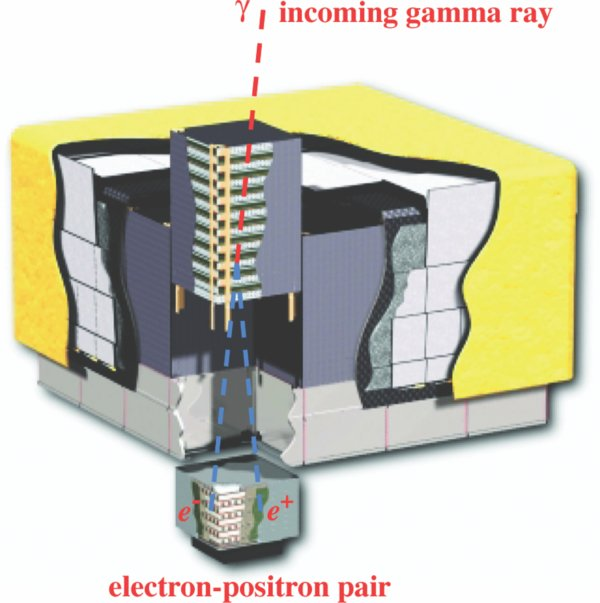
\includegraphics[width=0.6\textwidth]{chap/introduction/fig/fermi_lat.jpg}
	\caption{FERMI-LAT的结构示意图(引自\parencite{glast}),外包络尺寸为$1.8m \times 1.8m \times 0.72m$}
	\label{fig:introduction:fermi_lat}
\end{figure}


AMS-02是一个功能完备的大型磁谱仪,安装在国际空间站外部模块上。
AMS-02的具体结构见图\ref{fig:introduction:ams02},自上而下分别为:硅径迹探测器(Silicon Tracker),穿越辐射探测器(TRD),飞行时间探测器(TOF),永磁体,环像切连科夫探测器(RICH)和电磁量能器(ECAL)。其中,硅径迹探测器共有9层,其中2—8层径迹探测器在永磁体中,第1层和第9层分别靠近TRD和RICH。它主要测量的是入射宇宙线的轨迹,并结合永磁体得到磁刚度信息。TOF记录的是粒子到达的时间,据此可以判断宇宙线粒子是从哪个方向打进来的。知道了宇宙线粒子的方向和径迹,就知道了它在磁场中是怎么偏转的,据此可以判断宇宙线粒子所带的电荷的大小和正负。
\begin{figure}[htbp]
	\centering
	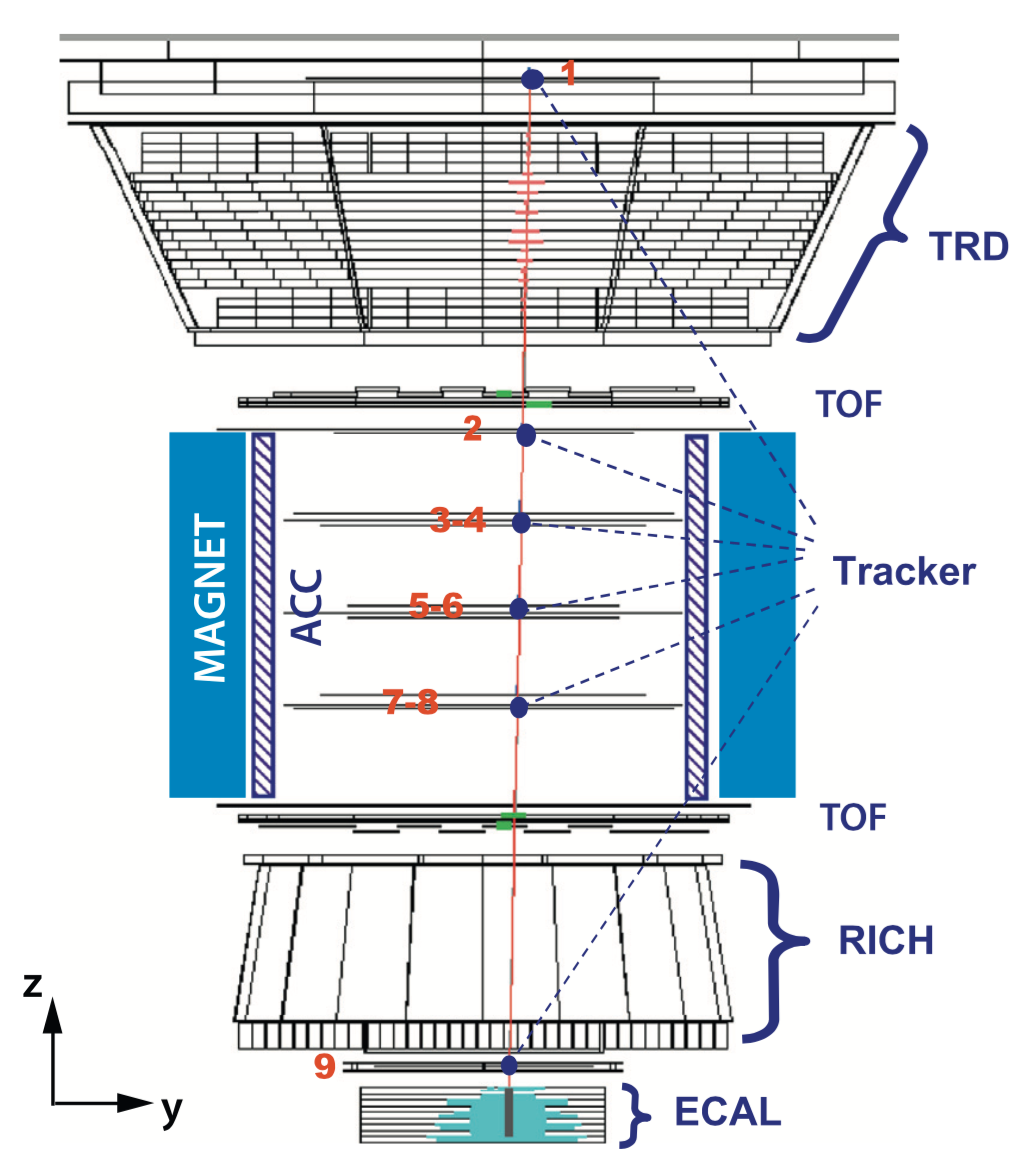
\includegraphics[width=0.6\textwidth]{chap/introduction/fig/ams022.png}
	\caption{AMS-02结构示意图(引自\parencite{ams02_detector})}
	\label{fig:introduction:ams02}
\end{figure}
TRD的主要功能是把高能正负电子从宇宙线中区分出来,而RICH用于测量入射宇宙线粒子的速度和电荷。
电磁量能器用于测量入射粒子能量。
自从2011年5月19日安装到国际空间站,一直到2015年4月15日,AMS02共累计了600亿的宇宙线事例。
AMS-02是迄今为止功能最强大、覆盖粒子种类最全面、测量精度最高的空间粒子探测器,将空间粒子探测提高到前所未有的一个新高度。


\section{暗物质粒子探测卫星简介}
暗物质粒子子探测卫星(DArk Matter Particle Explorer, 简称DAMPE)是中国科学院首批空间科学战略先导专项之一。
DAMPE粒子探测器是暗物质粒子探测卫星的主要载荷,它是一个高精度宽能段的能谱探测器,专门用来测量空间中高能电子、高能伽玛射线和重离子的能谱和分布。

\subsection{科学目标}
暗物质粒子探测卫星的科学目标可以归结为以下三个方面:
\begin{enumerate}
	\item 寻找暗物质粒子存在的证据,这是该项目的首要目标。通过在空间高分辨、宽能段地观测高能电子和伽玛射线寻找和研究暗物质粒子,间接测定其质量、湮灭截面或者寿命等重要的物理参量,并限定暗物质粒子的空间分布,在暗物质研究这一前沿科学领域取得重大突破。
	\item 宇宙线物理研究,通过测量TeV以上的高能电子能谱来研究宇宙线起源,通过测量TeV/核子的核素能谱来研究宇宙射线传播和加速机制。宇宙线的起源、加速传播机制是天文学中一个重要的研究课题。高能电子在星际中传播时,会与背景光发生逆康普顿散射且受星际磁场的作用发生同步辐射而损失能量,损失能量的速度与电子能量的平方成正比。能量越高的电子损失能量越快,所以高能电子不能够传播太远,地球附近的宇宙高能电子只能来自于附近的高能电子源,因此它被常用于研究宇宙线的起源。
	\item 伽玛射线天文学研究。DAMPE粒子探测器本身是一个高空间分辨和能量分辨的伽玛射线望远镜,其主要观测能段超过了国际上所有空间伽玛射线望远镜,可能会有许多预见不到的科学发现。
\end{enumerate}

    
\subsection{DAMPE粒子探测器的性能设计指标}

DAMPE粒子探测器的性能指标分为高能电子、高能伽马射线以及高能宇宙线重离子三个部分:
\begin{enumerate}
	\item 高能电子探测指标:
	\begin{itemize}
		\item 能区:$\SI{5}{GeV}\sim \SI{10}{TeV}$
		\item 能量分辨率:对于$\SI{800}{GeV}$的入射电子,达到\SI{1.5}{\percent}
		\item 空间分辨能力:对于$\SI{200}{GeV}$的入射电子,达到\SI{0.5}{\degree}
		\item 对质子本底的抑制能力:大于$10^5$
		\item 几何因子:大于$\SI{0.3}{m^2sr}$
	\end{itemize}
	\item 高能伽马射线探测指标:
	\begin{itemize}
		\item 能区:$\SI{5}{GeV}\sim \SI{10}{TeV}$
		\item 能量分辨率:对于$\SI{800}{GeV}$的入射伽马射线,达到\SI{1.5}{\percent}
		\item 空间分辨能力:对于$\SI{800}{GeV}$的入射伽马射线,达到\SI{0.5}{\degree}
		\item $e/\gamma$的分辨能力:大于$20$
		\item 几何因子:大于$\SI{0.2}{m^2sr}$
	\end{itemize}
	\item 宇宙线重离子探测指标:
	\begin{itemize}
		\item 能区:$\SI{100}{GeV}\sim \SI{100}{TeV}$
		\item 能量分辨率:对于$\SI{800}{GeV}$的入射重离子,大于\SI{40}{\percent}
		\item 空间分辨能力:对于$\SI{1}{TeV}$的入射重离子,达到\SI{1.0}{\degree}
		\item 几何因子:大于$\SI{0.2}{m^2sr}$
	\end{itemize}
\end{enumerate}
表\ref{tab:introduction:dampe_comparison}给出了DAMPE粒子探测器的主要性能参数与国际上其它同类探测器的比较,可以看到它的设计指标已经达到了国际先进水平。
% 卫星观测能段覆盖5GeV-10TeV,能量分辨优于1.5,超过国际上所有类似探测器。可望在暗物质粒子探测和宇宙线物理这两大科学难题上取得突破!同时更好的研究伽玛射线天文学等相关重要科学问题。

\begin{table}[htb]
	\centering
	\caption{DAMPE与其它同类探测器的性能比较}
	\label{tab:introduction:dampe_comparison}
	\begin{threeparttable}
	\begin{tabulary}{\linewidth}{LCCCC}
		\toprule[1.5pt]
		  & DAMPE & AMS-02 & FERMI-LAT & CALET \\ 
		\midrule[1pt]
		Energy Range (\si{GeV}) & $5\sim10^4$ & $0.1\sim10^3$ & $0.02\sim300$ & $1\sim10^3$ \\ 
		$e/\gamma$ Energy res.@\si{GeV}(\si{\percent}) & 1.5 & 3 & 10 & 2 \\ 
		$e/\gamma$ Angular res.@\si{GeV}(\si{\degree}) & 0.1 & 0.3 & 0.1 & 0.1 \\ 
		$e/p$ Discrimination& $10^5$ & $10^5\sim10^6$ & $10^3$ & $10^5$ \\ 
		Calorimeter thickness($\Psi_0$) & 31 & 17 & 8.6 & 30 \\ 
		Geometric accep.(\si{\meter\squared\steradian}) & 0.4 & 0.09 & 1 & 0.12 \\ 
		\bottomrule[1.5pt] 
	\end{tabulary}
	% \begin{tablenotes}
		% \item[*] DAMPE
	% \end{tablenotes}
	\end{threeparttable}
\end{table}

\subsection{DAMPE卫星的轨道、飞行程序与工作模式}

DAMPE卫星整体功耗为\SI{350}{W},重量为\SI{1400}{kg},设计寿命为三年\parencite{psd_tdr}。
它将运行于离地\SI{500}{\kilo\meter}的太阳同步轨道,轨道基本参数为:偏心率为0;轨道倾角为\SI{97.406}{\degree};轨道周期为95分钟;降交点地方时为UTC 6:30 AM。

图\ref{fig:introduction:flight_program}给出了DAMPE卫星的完整飞行程序。
\begin{figure}[htbp]
	\centering
	\includegraphics[width=0.95\textwidth]{chap/introduction/fig/flight_program.png}
	\caption{DAMPE卫星的飞行阶段划分(引自\parencite{psd_tdr})}
	\label{fig:introduction:flight_program}
\end{figure}
在完成对地捕获后,卫星开始进入两个月的在轨测试阶段,此时DAMPE粒子探测器正式加电进入工作模式。
测试阶段完成后,卫星就正式交付使用,进入科学观测阶段。
此时,DAMPE卫星主要具有以下两种工作模式:
\begin{itemize}
	\item 巡天探测模式。此阶段卫星姿态稳定对地,本体+Z轴指向地心,+X轴指向飞行方向,+Y轴指向轨道法向的反方向,使得DAMPE粒子探测器能够对全天区进行大范围观测。此阶段时间预计为2年。
	\item 定向探测模式。根据前一阶段巡天观测得到的数据,分析出暗物质可能存在的重点区域。此阶段卫星采用准惯性定向方式,对准重点区域或对准银心所在的维度进行准惯性观测。
\end{itemize}


\subsection{DAMPE粒子探测器的结构与组成}
DAMPE粒子探测器由四个子探测器系统组成,分别是塑闪阵列探测器,硅径迹探测器,BGO量能器和中子探测器,
图\ref{fig:introduction:dampe_structure}给出了它的结构示意图。
\begin{figure}[htb]
	\centering
	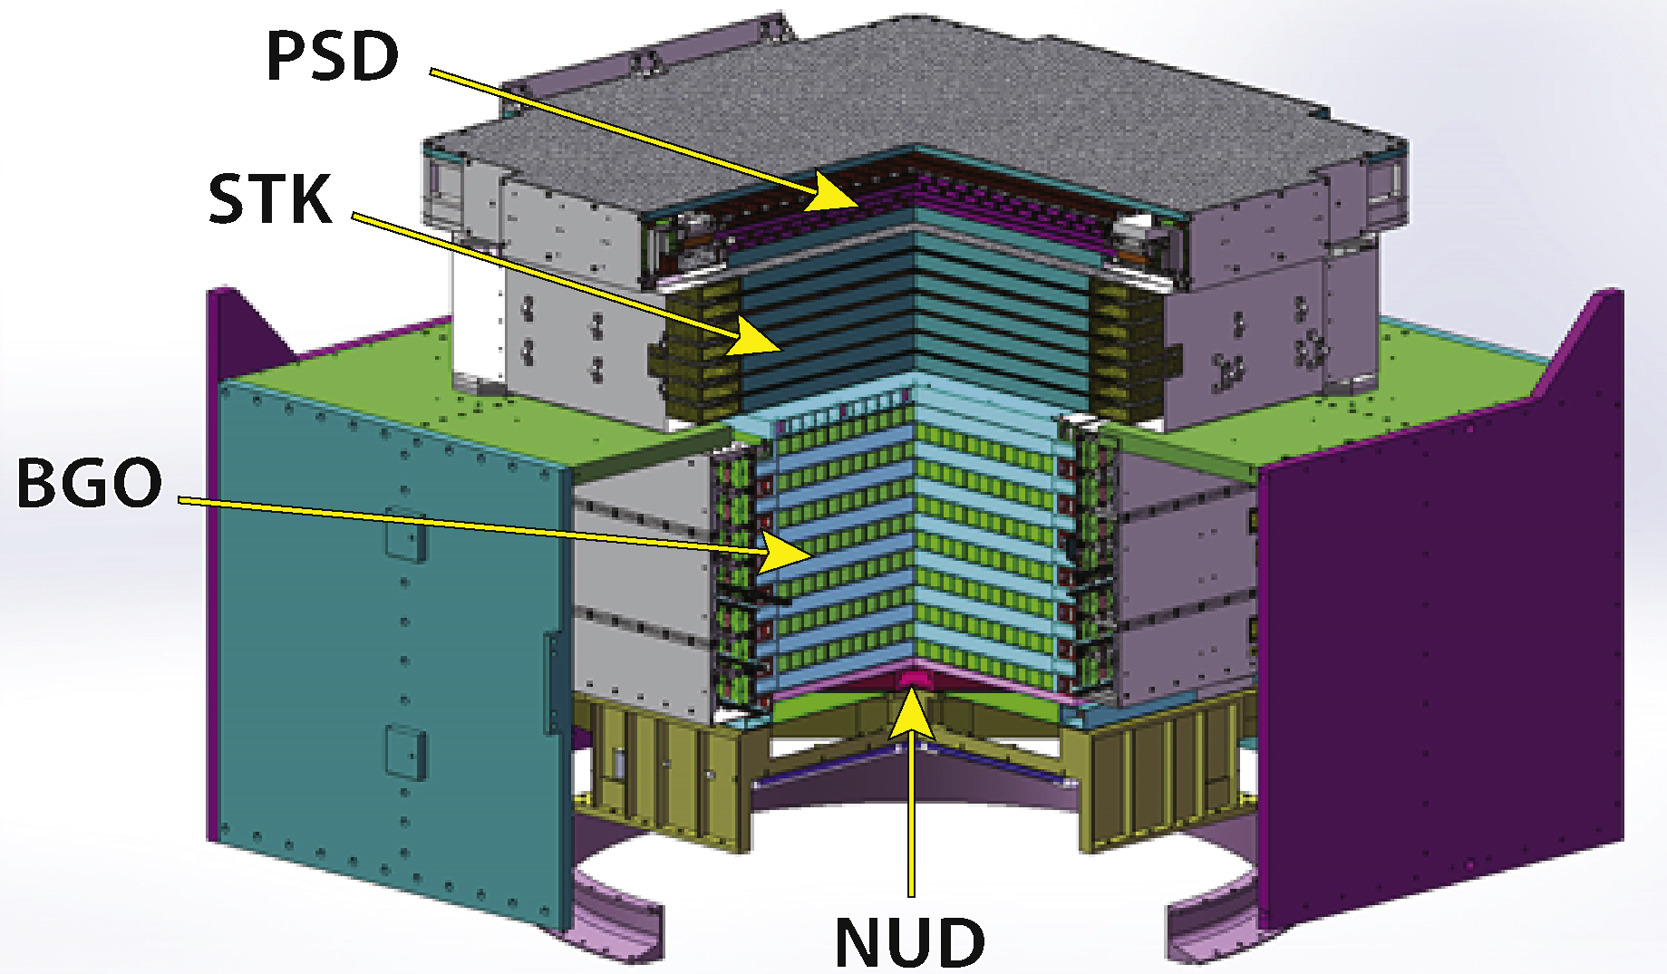
\includegraphics[width=0.8\linewidth]{chap/introduction/fig/dampe_structure}
	\caption{DAMPE暗物质粒子探测器的结构示意图(引自\parencite{psd_tdr})}
	\label{fig:introduction:dampe_structure}
\end{figure}


塑闪阵列探测器(Plastic Scintillator Array Detector,简称PSD)位于DAMPE卫星的最顶部,它的主要功能有:1)协助BGO量能器区分光子事件和电子事件;2)鉴别$Z=1\sim 20$的入射重离子,和硅径迹探测器电荷测量互为备份。
PSD由X、Y两层相互垂直的塑料闪烁体单元条平面阵列组成,有效探测面积为$820mm\times 820mm$。
PSD是本论文的主体内容,因此这里只对其进行简单介绍,有关PSD内部结构更详细的信息请参看第\ref{ch:description}章。

硅径迹探测器(Silicon-Tungsten Tracker,简称STK)位于PSD下方\parencite{stk_dampe},它的主要功能有:1)测量入射带电粒子的轨迹;2)利用电子对效应,将入射的高能$\gamma$转化为正负电子对,这一点和FERMI-LAT的设计类似;3)鉴别$Z=1\sim 26$入射重离子,和PSD的电荷测量互为备份。
STK的径迹探测和电荷测量由6层径迹探测平面完成(见图\ref{fig:introduction:stk_combined}(a)),每一层探测探测平面进一步由X、Y两个方向上的单面硅微条探测器组成。
其中,在第2,3,4层的径迹探测平面上还布置了\SI{1}{mm}的钨板,用于高能$\gamma$的转化。
每个单面硅微条探测器由16个Ladder组成,每个Ladder进一步由4块小的方形硅微条探测器串联而成,如图\ref{fig:introduction:stk_combined}(b)所示。
\begin{figure}[htbp]
	\centering
	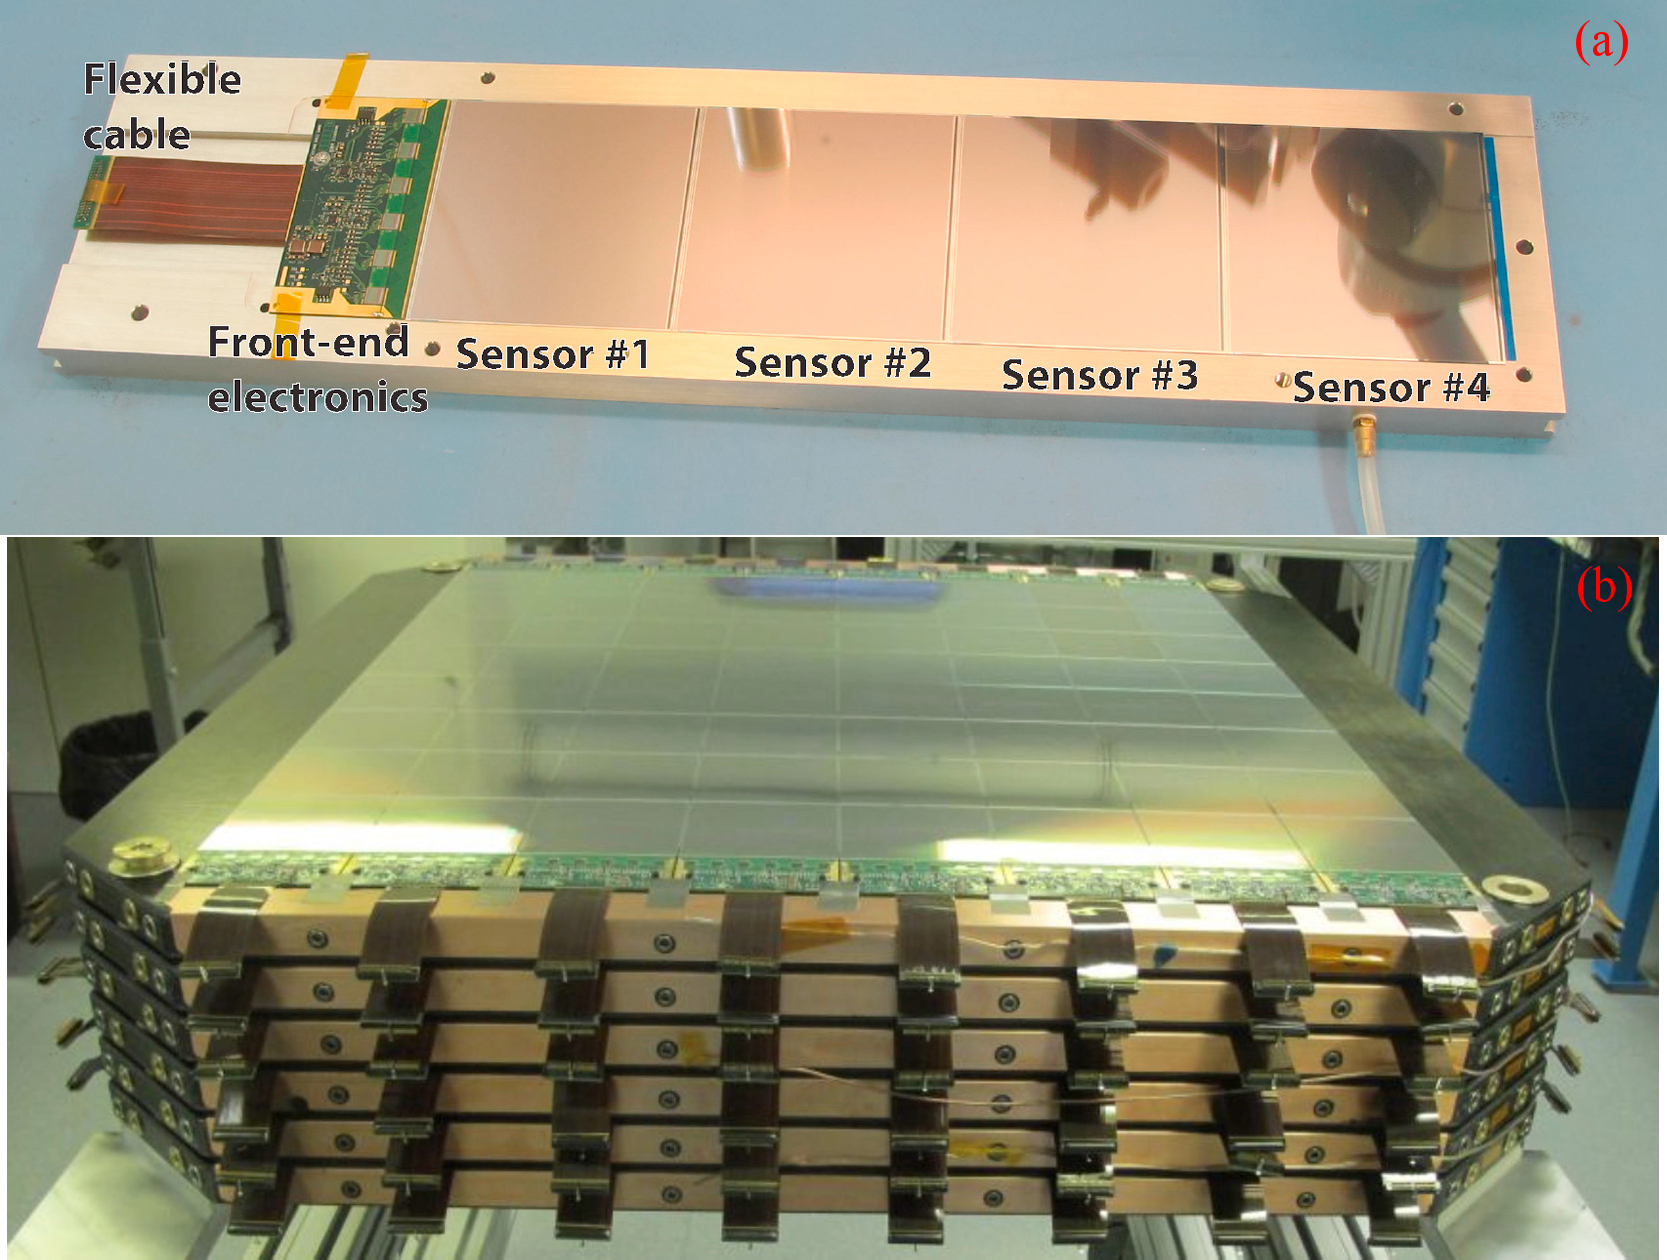
\includegraphics[width=0.7\textwidth]{chap/introduction/fig/stk_combined.jpg}
	\caption{a)STK的一个Ladder;b)组装完成后,STK的六层径迹探测平面(引自\parencite{stk_dampe})}
	\label{fig:introduction:stk_combined}
\end{figure}
这些小的硅微条探测器是STK的最小组成单元,其面积大小为$95mm\times 95mm$,因此可以得到整个STK的有效探测面积为$760mm \times 760mm$。
小型硅微条探测器的硅基地厚度为$\SI{320}{\micro\meter}$,上面分布有768路宽度为$\SI{121}{\micro\meter}$的硅微条。
STK对硅微条探测器的读出方式为隔条读出,因此每个Ladder具有389路输出信号,而整个STK共有73728路输出信号。
由于记录了输出信号的幅度信息,STK可以采用电荷分配的方法对击中位置进行重建。
对于所有的入射角度,STK的位置测量精度可以达到\SI{80}{\micro\meter},而当入射角度小于\SI{40}{\degree}时,甚至可以达到\SI{50}{\micro\meter}。

BGO量能器(BGO Calorimeter,简称BGO)位于卫星的中部\parencite{bgo_zhangzhiyong_thesis},它是DAMPE粒子探测器主体功能模块,用于对所有入射宇宙线粒子尤其是高能电子和高能伽马射线的能量进行测量。
另外,利用电磁簇射和强子簇射在量能器内部横向发展和纵向发展的不同,BGO可以用于强子(主要是质子)和$e/\gamma$的粒子鉴别,同时结合PSD的反符合功能完成$e$和$\gamma$的鉴别。
最后,BGO也将为DAMPE粒子探测器的提供触发信号,从而有效降低宇宙线本底质子事例的触发率。
BGO量能器由14层锗酸铋晶体阵列组成(见图\ref{fig:introduction:bgo}),约对应31个辐射长度和1.6个核作用长度。
\begin{figure}[htbp]
	\centering
	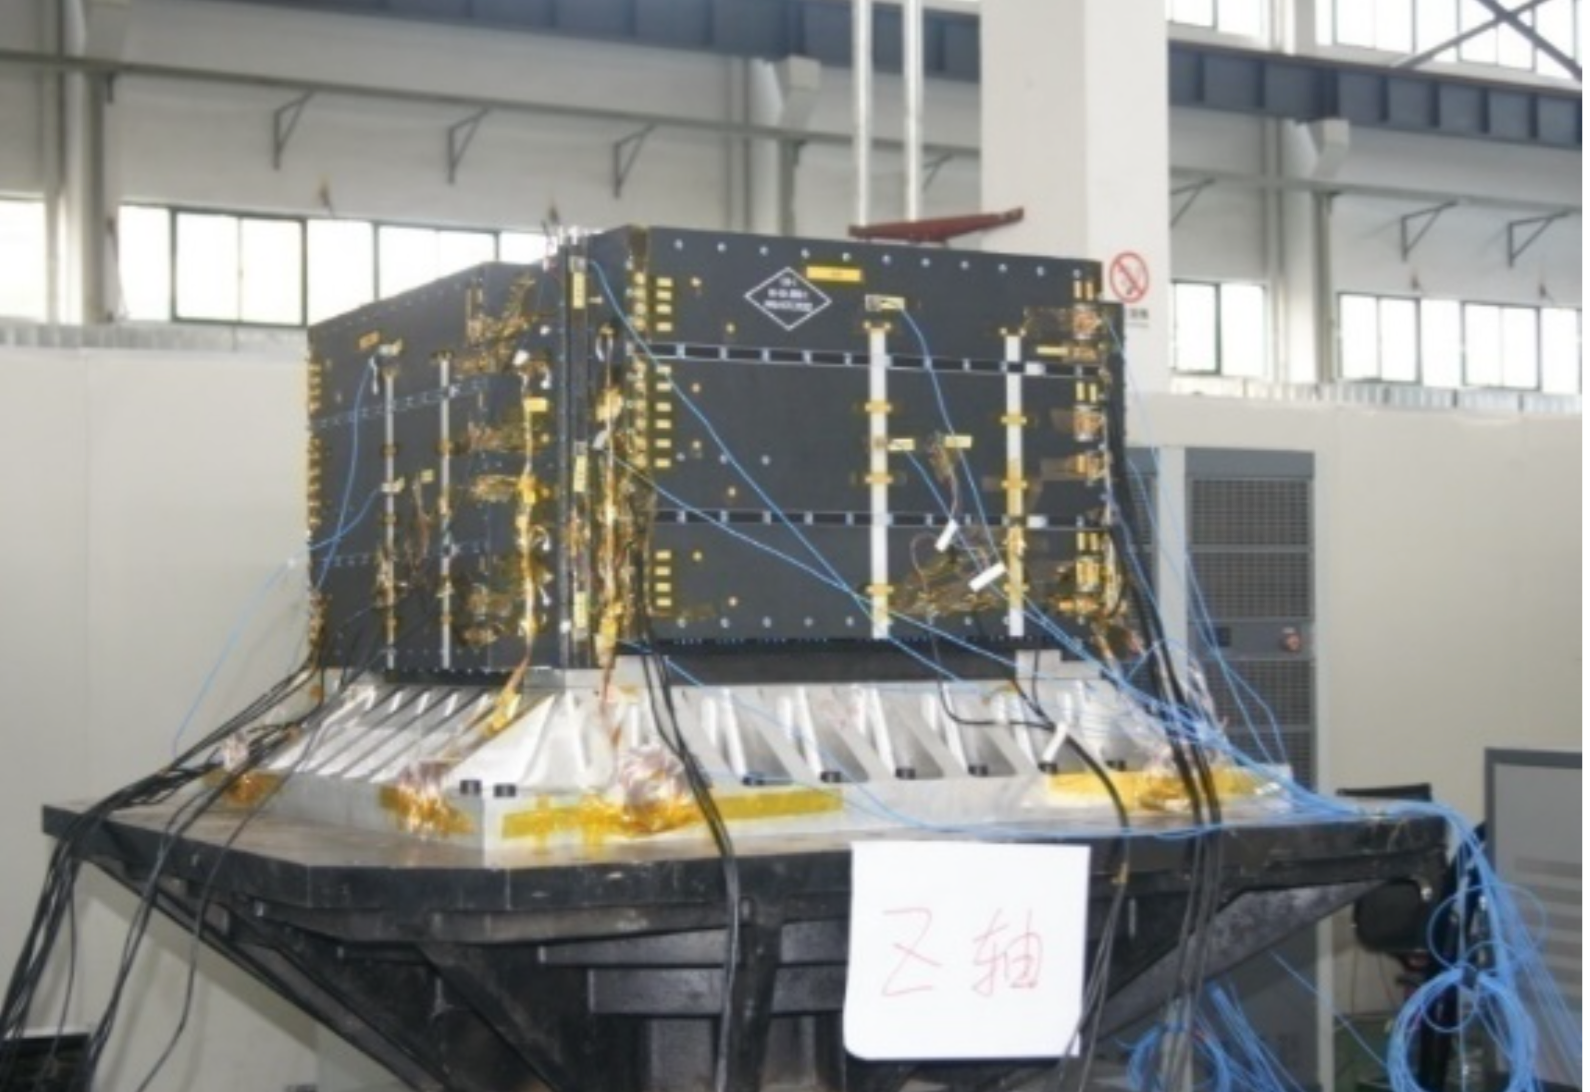
\includegraphics[width=0.65\textwidth]{chap/introduction/fig/bgo.png}
	\caption{在振动台上等待力学测试的BGO量能器}
	\label{fig:introduction:bgo}
\end{figure}

\begin{figure}[!htbp]
	\centering
	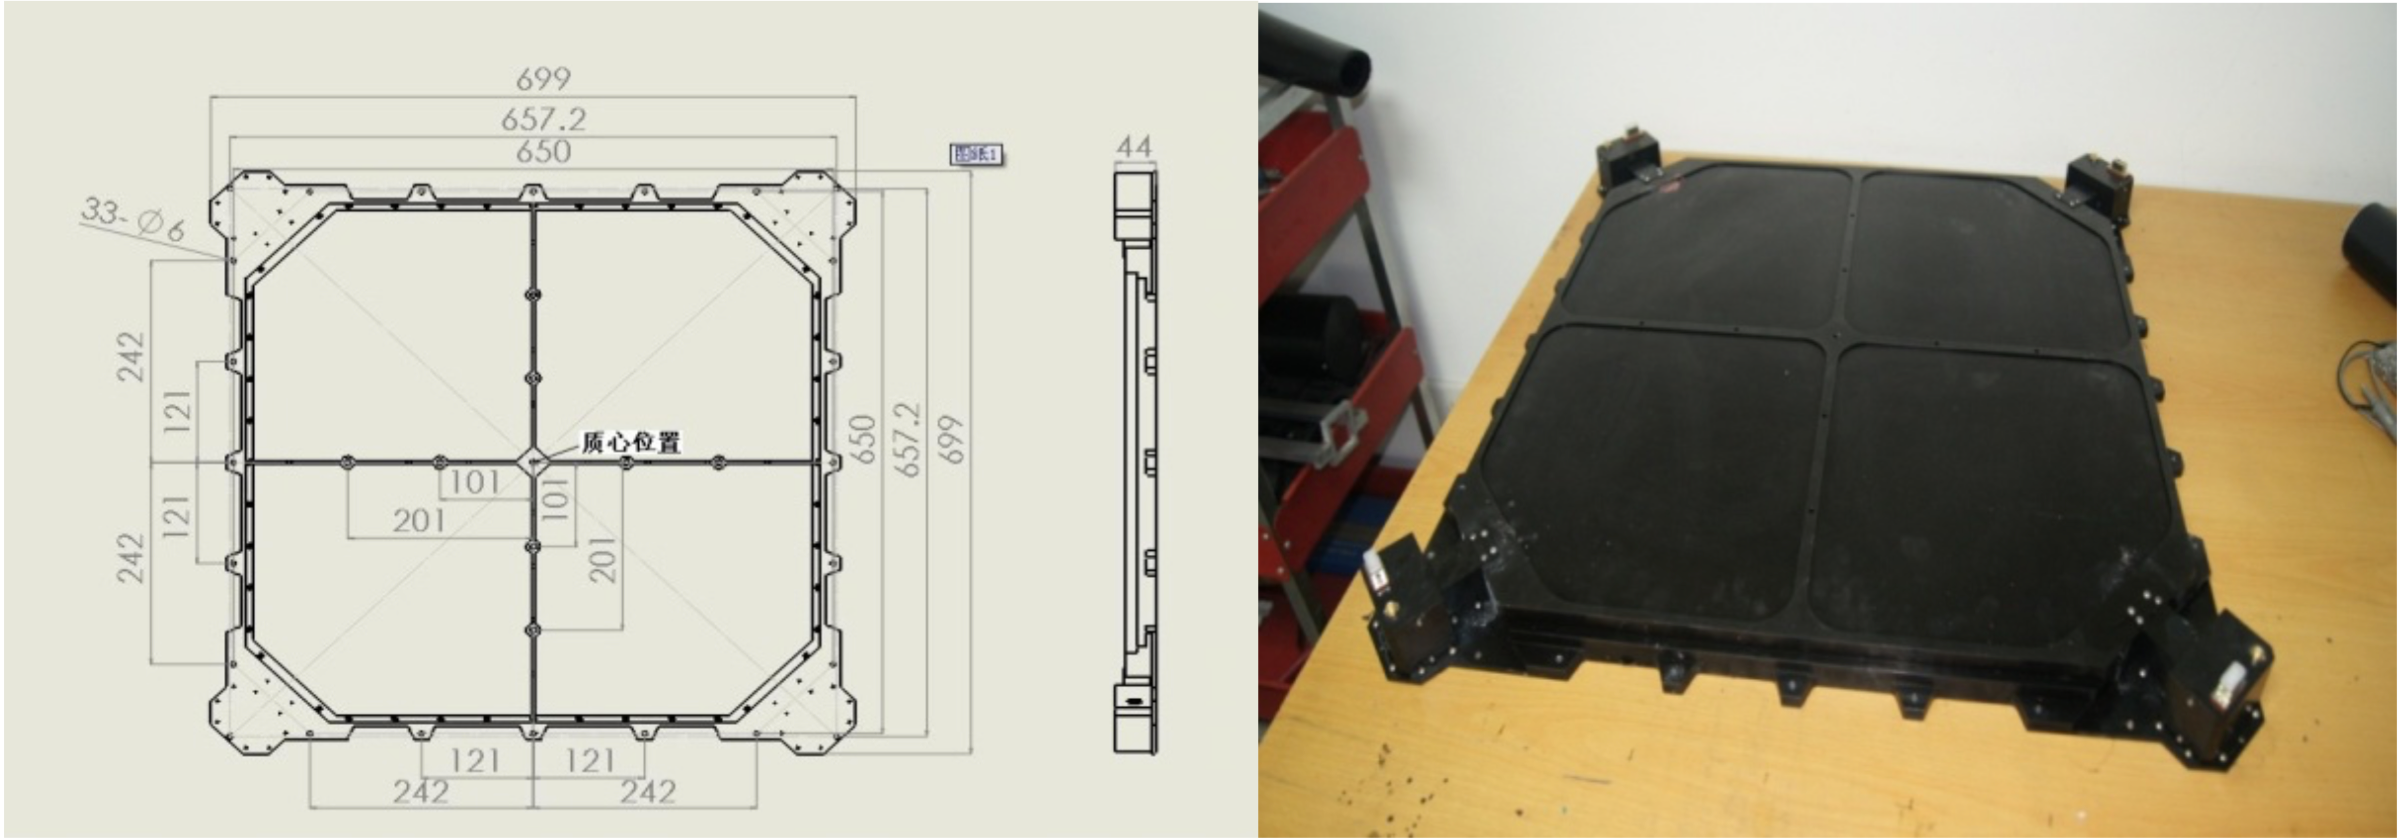
\includegraphics[width=0.9\textwidth]{chap/introduction/fig/nud.png}
	\caption{中子探测器的机械设计图与组装前的实物照片}
	\label{fig:introduction:nud}
\end{figure}
每层晶体阵列由22根尺寸为$25mm\times 25mm \times 600mm$的晶体单元条紧密排列而成,且相邻两层晶体阵列的排列方向相互垂直,以提供簇射发展的X-Y位置信息,从而形成一个三维的图像量能器。
BGO量能器采用双端读出的方法,在每根单元条两端各耦合一支光电倍增管,用于闪烁光信号的读出。
因此,BGO量能器一共使用308根BGO晶体和616支光电倍增管。


中子探测器(Neutron Detector,简称NUD)位于卫星最底部\parencite{changjin_introduction_2014},它的主要功能是测量宇宙线中的强子(主要为质子)与NUD前面的探测器物质(主要是BGO量能器)发生作用产生的次级中子。
高能质子在BGO中的强子簇射会产生大量的高能中子,而高能电子主要是电磁簇射,产生的中子数目很少,通过判断NUD内是否有能量沉积,可以进一步提高BGO鉴别质子和电子的能力\parencite{changjin_nud_2015}。
NUD采用厚度为\SI{10}{mm}的掺硼塑料闪烁体作为探测介质,有效探测面积为$\SI{693}{mm}\times\SI{693}{mm}$。
它由四块独立的正方形塑闪烁体构成其探测整体,并且每块塑料闪烁体都分别去除一个角以耦合一个光电倍增管进行信号读出,如图\ref{fig:introduction:nud}所示。
